\documentclass[a4paper]{article}
\usepackage{iwslt15,amssymb,amsmath,epsfig}
\usepackage{verbatim}
\usepackage{CJKutf8}
\usepackage{multirow}
\usepackage{newfloat}


\DeclareFloatingEnvironment[placement={!ht},name=Example]{mylist}
\newcommand{\ch}[1]{\begin{CJK}{UTF8}{gbsn}{#1}\end{CJK}}
\newcommand{\uch}[2]{\underbrace{\text{\ch{#1}}}_{\text{\ch{#2}}}}
%\newcommand{\anony}[1]{\textit{[anonymized]}}
\setcounter{page}{1}
\sloppy		% better line breaks
%\ninept
%SM below a registered trademark definition
\def\reg{{\rm\ooalign{\hfil
     \raise.07ex\hbox{\scriptsize R}\hfil\crcr\mathhexbox20D}}}

%% \newcommand{\reg}{\textsuperscript{\textcircled{\textsc r}}}

\title{Integrating Encyclopedic Knowledge into Neural Language Models}

%%%%%%%%%%%%%%%%%%%%%%%%%%%%%%%%%%%%%%%%%%%%%%%%%%%%%%%%%%%%%%%%%%%%%%%%%%
%% Please make sure to keep technical paper submissions anonymous  !
%%%%%%%%%%%%%%%%%%%%%%%%%%%%%%%%%%%%%%%%%%%%%%%%%%%%%%%%%%%%%%%%%%%%%%%%%%
%%%%%%%%%%%%%%%%%%%%%%%%%%%%%%%%%%%%%%%%%%%%%%%%%%%%%%%%%%%%%%%%%%%%%%%%%%
%% If multiple authors, uncomment and edit the lines shown below.       %%
%% Note that each line must be emphasized {\em } by itself.             %%
%% (by Stephen Martucci, author of spconf.sty).                         %%
%%%%%%%%%%%%%%%%%%%%%%%%%%%%%%%%%%%%%%%%%%%%%%%%%%%%%%%%%%%%%%%%%%%%%%%%%%
\makeatletter
\def\name#1{\gdef\@name{#1\\}}
 \makeatother
 \name{{\em Yang Zhang, Jan Niehues, Alexander Waibel}}
%%%%%%%%%%%%%%% End of required multiple authors changes %%%%%%%%%%%%%%%%%

\address{Institute for Anthropomatics  \\
Karlsruhe Institute of Technology, Germany \\
{\small \tt firstname.lastname@kit.edu}
}
%

\begin{document}

\maketitle
%
\begin{abstract}
Neural models have recently shown big improvements in the performance of phrase-based machine translation. Recurrent language models, in particular, have been a great success due to their ability to model arbitrary long context. In this work, we integrate global semantic information extracted from large encyclopedic sources into neural network language models. We integrate semantic word classes extracted from Wikipedia and sentence level topic information into an recurrent neural network-based language model.
The new resulting models exhibit great potential in alleviating data sparsity problems with the additional knowledge provided. This approach of integrating global information is not restricted to language modeling but can also be easily applied to any model that profits from context or further data resources, e.g. neural machine translation. Using this model has improved rescoring quality of a state-of-the-art phrase-based translation system by 0.84 BLEU points. We performed experiments on two language pairs.



\end{abstract}


%
\section{Introduction}
Recurrent neural network language models (RNNLMs) have recently shown great improvements in statistical machine translation (SMT), both during decoding and rescoring. The use of continuous word representations has achieved better generalization of the data which effectively lowered data sparsity problems. Furthermore, the recurrent connections are able to model long-range dependencies. Yet, most of these models strictly depend on monolingual and parallel data, which is sometimes not available in large amounts or only for specific domains, especially with low-resource languages.
This has motivated RNNLMs to take multiple parallel streams of data as input instead of just the single stream of surface words. These so-called factors can be used to add additional information, e.g. part-of-speech (POS) or automatic word clusters, which helps mainly with morphologically rich languages (e.g. Romanian, German). However, so far the additional factors were only limited to syntactic or local context information preceding the current word. Especially for languages without sufficient training data it is important to take advantage of other knowledge sources, e.g. encyclopedia. For example, Wikipedia has become a growing source for learning general concepts since the emergence of the Internet has led to an explosion of textual data. 
In this paper, we studied the integration of large encyclopedia sources into RNNLMs by using two approaches. 
In the first approach we use a factored model to integrate Wikipedia categories. 

In order to understand large unstructured data sets great achievements have been made in latent concept learning in the area of information retrieval. Techniques that categorize documents include latent semantic analysis and probabilistic topic modeling. In the second approach, we use term frequency–inverse document frequency (tf-idf), latent semantic analysis (LSA) and latent Dirichlet allocation (LDA) to compute a real-valued topic vector for each sentence that is fed as an additional input into the network. 

These approaches utilize external word categories and topic information in addition to the local contexts implicitly provided by recurrent neural models to improve lexical selection. 


\section{Related work}
Language models are a critical component of many application systems, e.g. automatic speech recognition, machine translation and optical character recognition. However, language models have always faced the problem of data sparsity. Factored language models \cite{bilmes2003factored} introduced the use of a bundle of factors associated with a word which outperformed previous $n$-gram models without expanding the training data. In the work of \cite{bilmes2003factored} morphs, stems, POS and clustered word classes were used as factors. In \cite{koehn2007factored}, the single feature stream of surface words was replaced with multiple factors and integrated into a phrase-based SMT system by breaking down the translation model into several steps that pertain to the translation of single factors, which again influence the prediction of the next word.
After recurrent neural network models became a success in language modeling \cite{mikolov2010recurrent}, a factored input layer was employed in a model by \cite{wu2012factored} which uses a structured output layer based on word classes to handle vocabularies of large size.
Motivated by multi-task learning in natural language processing, \cite{niehuesusing} proposed a multi-factor recurrent neural network language model (FRNNLM) which jointly predicts different output factors by mapping the output of the LSTM-layer \cite{hochreiter1997long} to as many softmax layers as there are output factors, thereby creating multiple distributions at the output layer. In the rescoring of $n$-best lists, this model can be included as either one or several additional features depending on whether the output is treated as a joint probability or individual probabilities.
Compared to a fixed-length factored input, a dedicated continuous space vector offers more flexibility and possibility to integrate additional side information, e.g. topic information. In \cite{mikolov2012context}, an approach to use an additional input vector in a neural language model was proposed. In their work, a vector instead of a single factor is associated with each word. However, this vector depends only on a word's earlier local context, thus neglecting the influence of the future context on a word's meaning. 
Often, the meaning of a word cannot be just derived from its preceding words but depends on the content words of the entire sentence or surrounding sentences. 
Topic models play a great role in information retrieval because they summarize large amounts of documents into fewer concepts by capturing word co-occurrence information. Essentially, topic models can be divided into vector space models (VSMs), e.g. LSA \cite{deerwester1990indexing}, and probability models, e.g. LDA \cite{blei2003latent}. 
The successful usage of Wikipedia to devise methods for computing semantic relatedness of documents was reported in \cite{gabrilovich2007computing} and \cite{strube2006wikirelate}.
Generative probabilistic models were employed in \cite{han2012entity} to link named entities in text documents by using information extracted from Wikipedia. 
In \cite{cucerzan2007large} and \cite{bunescu2006using} VSMs were employed to resolve word disambiguations based on entities derived from Wikipedia.
Similar methods were applied to other knowledge sources, such as WordNet \cite{hearst1992automatic}.
However, to our knowledge, it is the first time encyclopedic knowledge is used to supplement neural language modeling.

\section{Integration of encyclopedic information}
We propose two approaches to integrate encyclopedic information into neural language models of the target side of a language pair.
First, the target side words are labeled with Wikipedia categories. The hierarchical page structure of Wikipedia in the target language enables us to obtain a page's category which we use as factored input into the previously described FRNNLM.
Second, for every sentence in the data a ranking of related encyclopedia articles is established by using a VSM or topic model. Based on the underlying model, a feature vector, which comprises the information of the most similar documents to the current sentence, is computed  and fed into a neural language model as additional input. The second approach is not limited to Wikipedia, but can be applied to any encyclopedia. To test the performance of this method independently of the underlying knowledge source we have crawled a Chinese lexicon from zdic.net \cite{zdic} with 38.285 articles, for which the results are presented later on. 


\subsection{Word-level information} \label{sec:word-level}
The motivation behind using word categories from Wikipedia in association with words is to strengthen the relatedness of words in the same correct translation hypothesis to prevent it from being discarded due to a low translation score.
Let's look at an example source sentence:
\begin{align*}
\text{``A journalist writes articles for a column''}
\end{align*}
Both of the following hypotheses, as shown in Example \ref{ex:wiki-cat}, are possible translation hypotheses:
\begin{mylist}
\caption{\it Two hypotheses whose nouns are labeled with Wikipedia categories.}
\newcommand{\uchx}[3]{\underbrace{\substack{\text{\ch{#1}}\\\text{#2}}}_{\text{\ch{#3}}}}
\begin{center}
\begin{minipage}{200pt}
\begin{enumerate}
\item $\uchx{一位}{one}{NR}$ $\uchx{记者}{journalist}{新闻 (=news)}$ $\uchx{给}{for}{P}$ $\uchx{柱子}{column}{建筑(=archit.)}$ $\uchx{写}{write}{VV}$ $\uchx{文章}{article}{作品}$
\item $\uchx{一位}{one}{NR}$ $\uchx{记者}{journalist}{新闻 (=news)}$ $\uchx{给}{for}{P}$ $\uchx{专栏}{column}{新闻(=news)}$ $\uchx{写}{write}{VV}$ $\uchx{文章}{article}{作品}$
\end{enumerate}
\end{minipage}
\end{center}
\label{ex:wiki-cat}
\end{mylist}

Although the second translation is more accurate, because ``column'' in the context of ``journalist'' and ``article'' is translated with a newspaper section, the first translation could be more likely according to the translation model, since, generally, a column refers more often to a pillar than a newspaper section. In both translations, the translation of ``column'' is three words away from its next context word, the translation of ``article''. In a translation task where the data does not originate from news-related domains or is limited in size such that the words ``\ch{专栏 (=column)}'' and ``\ch{记者 (=journalist)}'' are never seen in the same context, the language model will fail to choose the correct translation.
Our approach solves this problem by labeling the words with according Wikipedia categories. By doing so, the bond between ``\ch{专栏 (=column)}'' and ``\ch{记者 (=journalist)}'' would be reinforced by their common factor ``\ch{新闻 (=news)}'', which contributes to a higher score of the correct translation. 



\subsubsection{Input representation}
We are only interested in Wikipedia pages, that are either an article or a category page.
We define the search space as the set of all Wikipedia pages of interest. Given a word, we search for the page with the same word as title and retrieve its category which is found at the bottom of the page.
In case of multiple categories we pick the first one.
In the implementation, the offline Wikipedia dump is used to create a mapping between pages and their categories. Using a lower bound for the number of elements in a category, we pick recursively the parent of a category if it does not meet this requirement. In the later experiments we used a lower bound of five. This reduces the total number of associated articles and leads to better performances. In case no category is found at all, a word's part-of-speech is used instead.
One characteristic of Wikipedia is that most of its articles only refer to a small group of lexical categories. For example, there are a lot more articles about objects (nouns) than activities (verbs). Since topic words are usually nouns, it suffices to label only nouns in a sentence to improve model quality, which is shown in Example \ref{ex:wiki-cat}.

\subsubsection{Factored neural language model}
To incorporate the Wikipedia factors, we trained FRNNLMs as proposed in \cite{niehuesusing}, which takes one or multiple factors at the input layer and offers the option of a factorized output layer. After concatenating the embeddings of the input factors into a single word embedding, this vector is sent through one or multiple LSTM-based layers \cite{hochreiter1997long} before projected onto the factored output probabilities. The instance of the model used for this work takes two factors, the surface form and the Wikipedia word category. These are mapped onto an embedding vector of size 100, which is the same size as the first LSTM-layer. For the second LSTM-layer 200 nodes are chosen. We defined only one output factor, which is the word's surface form.


\subsection{Sentence-level information} \label{sec:sentence-level}
The idea to use a dedicated topic vector is motivated by a more flexible representation of information and methods that are capable of drawing correlations betweens words independently of their distance.
For example, the sentence 
\begin{align*}
\text{``Columns contain articles written by journalists''}
\end{align*}
exhibits several problems. First, when a corpus is translated into a low-resource language, e.g. Romanian, some of the content words do not have their own Wikipedia entries. This means we cannot take full advantage of the first approach. Second, the main context word of ``columns'', which is ``journalists'', appears later in the sentence; therefore a recurrent language model that only considers the previous context would fail. 
This motivated the idea to consider words in the entire sentence, unlike \cite{mikolov2012context}, and create a topic vector for each sentence by searching through Wikipedia to find topic related articles. In the above example sentence, these would probably be news-related articles. By compressing the information of these articles into a vector which is associated with each word, external topic information spanning neighboring words can be considered when translating a word. 
To create a ranking of similar documents and their representation to a given sentence, VSMs can be employed, such as tf-idf \cite{salton1986introduction} and LSA \cite{bradford2008empirical}, but also probabilistic models, such as LDA \cite{blei2003latent}. After representing the sentences and cleaned encyclopedia documents $\text{D}=\{d_1, d_2, \ldots, d_M\}$ in vector form, where the vector entries index into a vocabulary $V=\{v_1, v_2, \ldots, v_N\}$, we query for each sentence $w= \{w_1, w_2, \ldots, w_l\}$ the $n$ most similar documents $\text{D}_n=\{d|\text{score}(s, d) > c\}$, where $c \in \mathbb{R}$ is a threshold such that $|\text{D}_n| = n$ and $\text{score}(s, d)$ is a similarity function characterized by chosen model. These documents provide topic-related information about the current sentence. $\text{D}_n$ are transformed into vector representations $\{h(d)| d \in \text{D}_n\}$, where the vector representation $h(d)$ is defined by the model, which can differ from that used for scoring. The average of the vectors forms an additional feature input $\text{f}$ for a recurrent neural network-based language model, which we will refer to as an extended recurrent neural language model (ERNNLM).
\begin{equation}
\label{eq:f}
\text{f}=\dfrac{\sum_{d \in \text{D}_n} h(d)}{|\text{D}_n|}
\end{equation}
 This process is illustrated in Figure \ref{fig:flow}.
 For the topic models we used the python library gensim \cite{gensimTo21:online}.
\begin{figure} 
\centering 
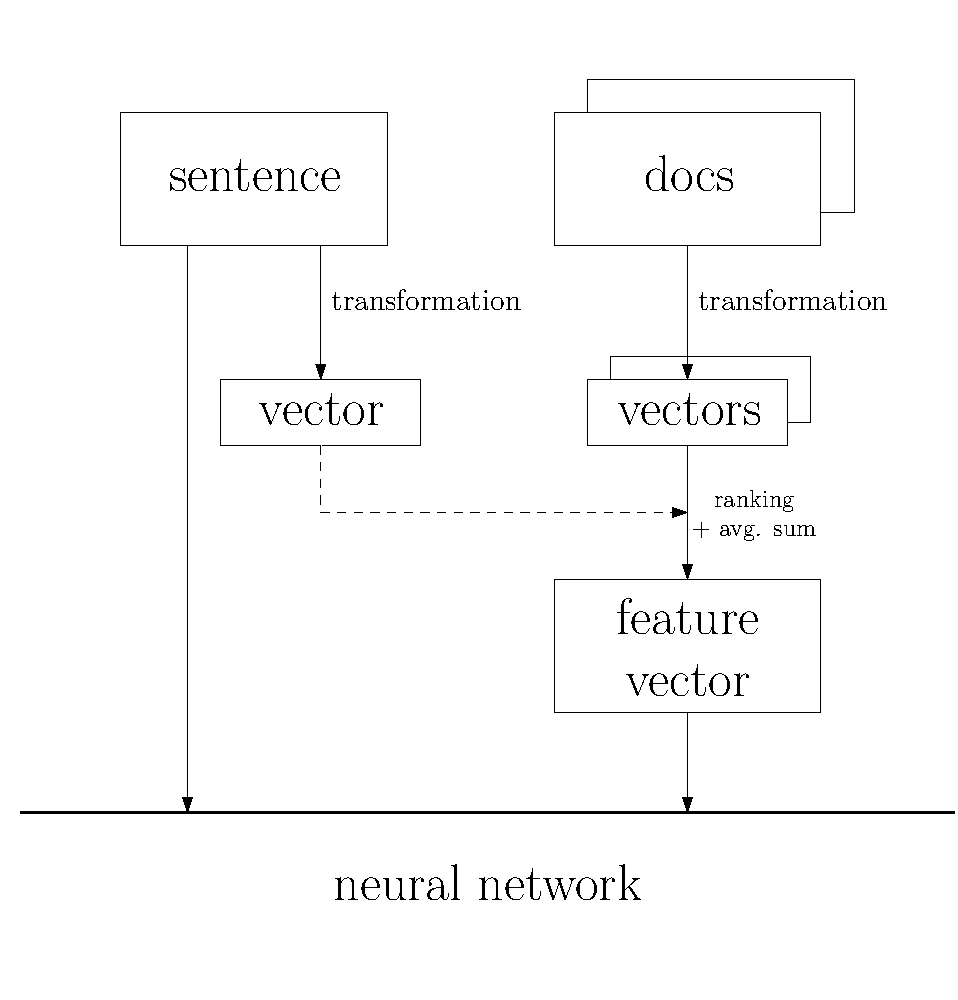
\includegraphics[width=\columnwidth]{flow.pdf}
\caption{\it Feature input creation process for the ERNNLM. Sentence and encyclopedia articles are transformed into vector representations based on the underlying method. The articles most similar to the sentence are chosen; their average constitutes the feature input.}
\label{fig:flow}
\end{figure}

\subsubsection{Tf-idf}
Tf-idf \cite{salton1986introduction} is a co-occurrence measure and determines the importance of a word to a set of documents $\text{D}$. Having the capability of grading down terms that appear in multiple documents, tf-idf is computed by multiplying a local component (term frequency or $tf$) with a global component (inverse document frequency or $idf$).
The cosine distance can be used to determine a ranking of similar documents for a given sentence query.
Shortcomings of this model include the inability to reduce the description length of the document, since words are only replaced by values.
Given a query sentence $w$ and a document $d$, we define the scoring function for this model as
\begin{equation}
\begin{aligned}
\label{eq:score_tfidf}
& \text{score}_{tfidf}(w, d) = \\ & \dfrac{\sum_{i=1}^{N} tfidf(v_i, w, \text{D}) \cdot tfidf(v_i, d, \text{D})} {\|\sum_{i=1}^{N} tfidf(v_i, w, \text{D}) \| \cdot \| \sum_{i=1}^{N} tfidf(v_i, d, \text{D})\|}
\end{aligned}
\end{equation}
The vector representation of a document is defined as
\begin{equation}
\label{eq:h_tfidf}
h_{tfidf}(d) = (tfidf(v_i, d))_{v_i \in V}
\end{equation}



\subsubsection{Latent semantic analysis}
LSA \cite{deerwester1990indexing} is a method that discovers hidden concepts in documents by using single value decomposition (SVD) on the set of documents $D$.
LSA uses a term-document matrix $A$, where the entry $A_{i,j}$ equates to the tf-idf value of the term $i$ for the document $j$. SVD decomposes $A$ into $U$, $\Sigma$, and $V$, such that $A = U \Sigma V^T$.
LSA uses the decomposition to find a low-rank approximation, that is, a matrix $A_k = U_k \Sigma_k V_k^T$ of a predefined lower rank $k$ closest in similarity to the original matrix $A$. This is done by deleting all but the $k$ biggest single values in $\Sigma$.
By doing so, LSA minimizes the Frobenius norm $\|A-A_k\|_F$. In this work, $k$ is the number of hidden concepts to be learned. The approximation of the $i$-th document vector in the low-dimensional space, denoted with $\hat{d_i}$, is the  $i$-th column of $V_k^T$.
The number of dimensions $k$ is an empirical question. Essentially, $k$ is much smaller than the original space dimension, which is usually the total number of documents. Previous papers show that for Wikipedia dumps a good value for $k$ should be chosen between 200 to 500 \cite{bradford2008empirical}. In this work $k$ is 300.
Given a sentence $w$ and a document $d$, we define the scoring function for this model as
\begin{equation}
\label{eq:score_lsi}
score_{lsa}(w, d) = \dfrac{\Sigma_k^{-1} U_k^T w * \hat{d}} {\|\Sigma_k^{-1} U_k^T w \| \cdot \| \hat{d}\|}
\end{equation}
The vector representation of a document is defined as
\begin{equation}
\label{eq:h_lsa}
h_{lsa}(d) = \hat{d}
\end{equation}


\subsubsection{Latent Dirichlet allocation}
LDA \cite{blei2003latent} is a generative probabilistic model that discovers automatically topics from a data collection.
The basic idea is that documents are represented as random mixtures over latent topics, where each topic is characterized by a distribution over words. The model is a three-level hierarchical Bayesian model with the first level being the corpus-level, the second being the document-level, and the third being the word-level. Setting the number of topics to be learned to $k$, learning is performed with variational Bayesian inference in combination with the EM algorithm. As for K, \cite{hoffman2010online} discusses how to choose the number of topics. In this work $k$ is 100, which is also the size of the feature vector.
Given a sentence $w$ and a document $d$, we defined the scoring function for this model as
\begin{equation}
\label{eq:score_lda}
 score_{lda}(w, d) = P(w|\theta_d, \alpha, \beta),
\end{equation}
where $\theta$, $\alpha$ and $\beta$ are parameters denoted and estimated as in \cite{hoffman2010online}.
The vector representation of a document is defined as
\begin{equation}
\label{eq:h_lda}
h_{lda}(d) = \theta_d
\end{equation}


\subsubsection{Extended language model}
The basic RNNLM consists of an input layer, a hidden layer with recurrent connections that maintains a representation of the sentence history, and an output layer which produces the probability distribution over words.
The ERNNLM, illustrated in \ref{fig:model-extended}, extends the RNNLM with an additional sentence-based feature layer that is connected to the output layer. Since this real-valued feature vector stays the same for all words in the current sentence, it is replicated for each word. This way, the feature information is retained in the model while the same sentence is being processed.
The $m$ hidden layers are based on LSTMs \cite{hochreiter1997long}.
Given a sentence $w = \{w_1, w_2, \ldots, w_l\}$, the sentence-level information $\text{f}$ is computed according to \eqref{eq:f} and duplicated for each word. For the $i$-th word we denote its 1-of-N representation with $x_i$, the hidden layers with $s^1, s^2, \dots, s^m$ and the output layer with $y_i$. The hidden and output layers are computed according to \eqref{eq}.
\begin{equation}
\label{eq}
\begin{aligned}
s^1_i &= f_1(U_1x_i + W_1s^1_{i-1}) \\
s^j_i &= f_j(U_js^{j-1}_i + W_js^j_{i-1}), \\j &\in \{2,\ldots,m\} \\
y_i &= g(Vs^m_i + F\text{f})
\end{aligned}
\end{equation}
where $f_i$ represents activation functions, and $g$ the softmax function.
To train the network, that is to find the weight matrices $U_{1,\dots,m}, V, W_{1,\dots,m}, F$, stochastic gradient descent is used according to the negative log-likelihood loss function. We also tested the option of adding an additional connection from the feature layer to the first hidden layer, which is illustrated in Figure \ref{fig:model-extended}.

\begin{figure} 
\centering 
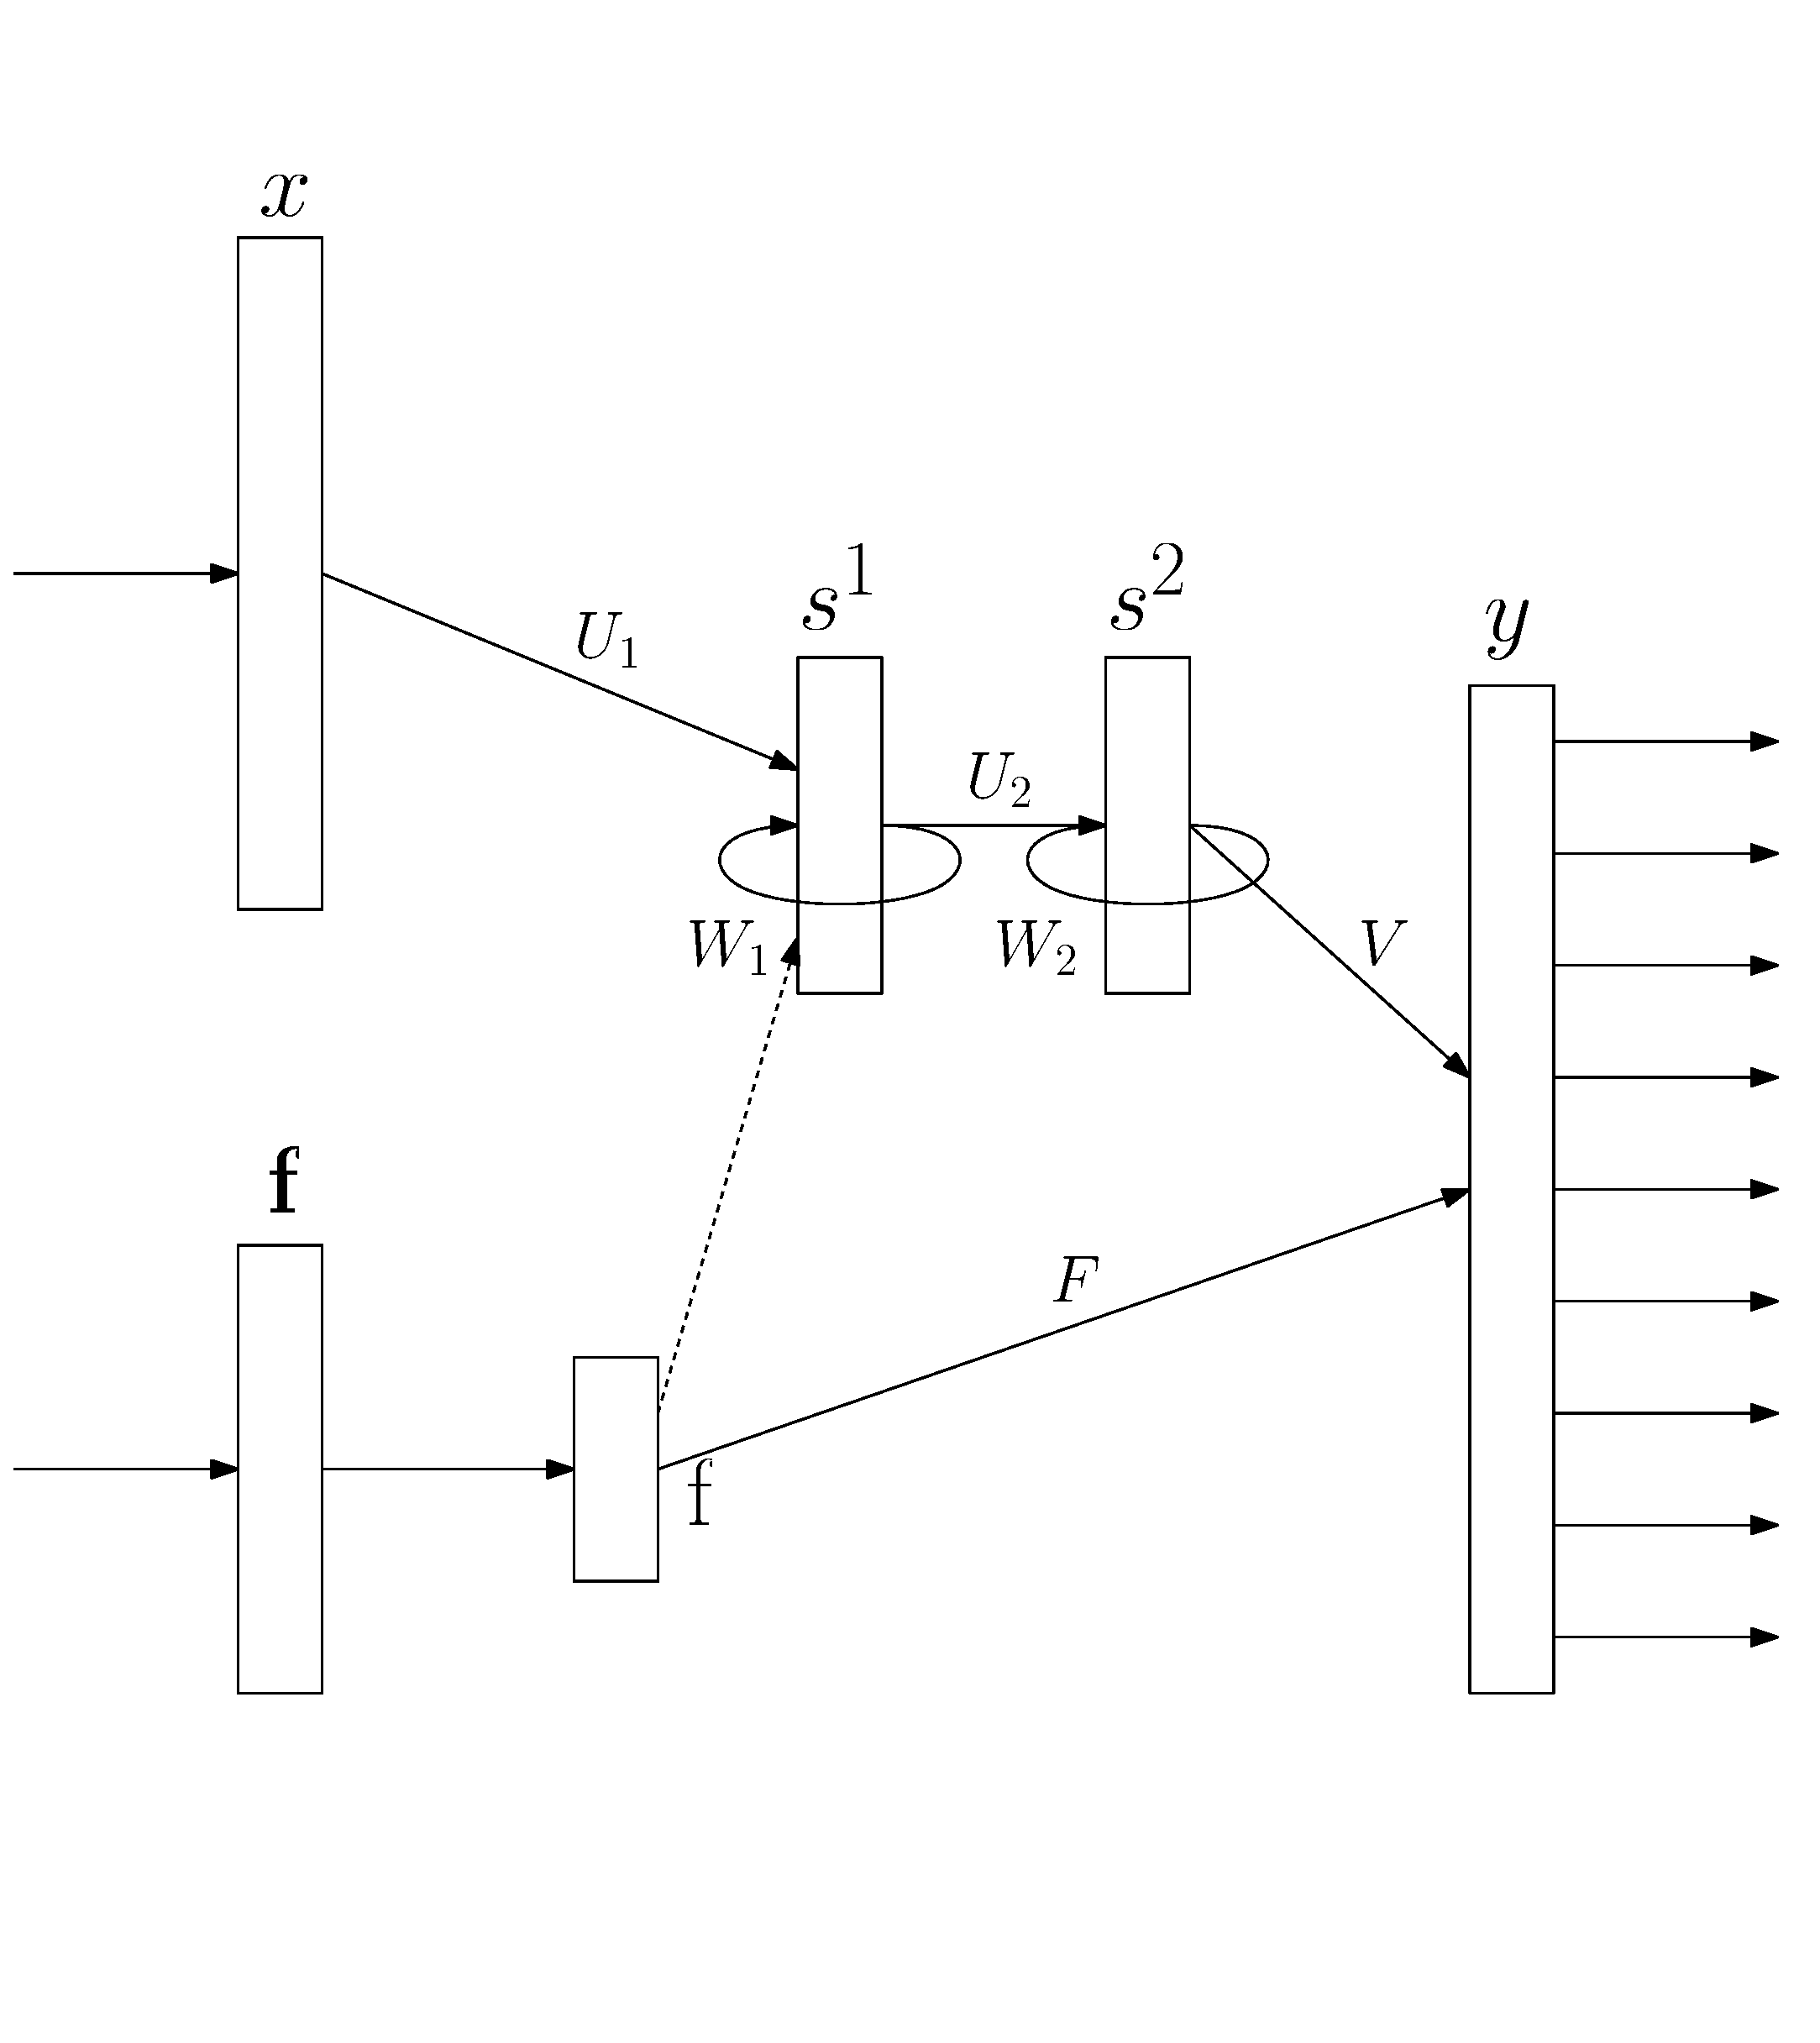
\includegraphics[width=\columnwidth]{ModelExtended2.pdf}
\caption{\it ERNNLM with additional feature input $\textbf{f}$ and two LSTM-based hidden layers. The dashed line from the feature input to the first hidden layer represents an optional connection.}
\label{fig:model-extended}
\end{figure}


\section{Experiments}
We evaluated both the FRNNLM and the ERNNLM on English-Chinese (ZH) and English-Romanian (RO) language pairs. For each language pair $n$-best lists are created with our in-house phrase-based MT system; the models are used as additional features in rescoring.

\subsection{System description}
The baseline system is an in-house implementation of a phrase-based MT system and is used to generate $n$-best lists on all of the available training data. The ZH-system is trained on the TED and UN corpus, optimized and rescored on the TED dev2010 and tested on the test2010 corpora. The Chinese corpus contains 148.968 sentences, the development set 887 sentences. The Chinese neural language models are tested on a $3000$-best list with a total of 455.965 sentences.
The RO-system is trained on the corpora of WMT 2015 Shared Translation Task, optimized on the first half of news-dev 2016 and tested on the second half of news-dev 2016. In addition, a subset of 2000 sentences of the SETimes corpus is used for further optimization in rescoring. The Romanian corpus contains 604.588 sentences, the development set 1000 sentences. The Romanian neural language models are tested in three configurations on $300$-best lists with 1.288.319, 167.567 and 162.928 sentences respectively.

The ZH-baseline system uses two word-based language models, and 12 features in total to create a $3000$-best list.
The RO-baseline system uses two word-based language models, two cluster-based models using 50, 100 or 1000 clusters, and a POS-based language model. In total 22-23 features are used to generate a $300$-best list. A full system description can be found in \cite{niehuesusing}.
In decoding, both language pairs are optimized with minimum error rate training (MERT) \cite{och2003minimum}. The same is used for rescoring of the ZH-system, whereas the RO-system uses ListNet to rerank the $n$-best list.
Both FRNNLMs and ERNNLMs for both language pairs are trained on the target side of the parallel training data. The Chinese neural language models use a vocabulary of 10K, while the Romanian models use a vocabulary of 5K. Wikipedia is used to obtain word-level side information, as described in Section \ref{sec:word-level}.
To gather sentence-level topic information for the ZH-system, as described in \ref{sec:sentence-level}, we additionally web-crawled a Chinese lexicon from zdic.net \cite{zdic} to show the model's performance independently of a specific encyclopedia.


\subsection{English-Chinese}
The ZH-system before rescoring gives a BLEU score 17.02 in testing. For all of the following experiments, our baseline system is rescored with a basic RNNLM.
In the first ZH-experiment we used the scores of the FRNNLM in addition to the baseline features, which is shown in Table \ref{tb:zh-factored}. Only nouns in the data are labeled with Wikipedia categories, which leads to 11.21 \% coverage of the development set and 10.61 \% of the test set. The FRNNLM that uses words and Wikipedia categories as factors causes an increase of 0.66 BLEU in testing compared to the same model without Wikipedia categories. The system that uses words, Wikipedia categories, and POS as factors performs 0.84 BLEU points better than the same system without the use of Wikipedia categories.

\begin{table}
\caption{\it ZH-FRNNLM}
\vspace{2mm}
\centering
  \begin{tabular}{ lll }
  	\hline
  	Model                 & devdata       & testdata      \\ \hline\hline
  	%Baseline             & 14.69         & 17.05         \\
  	Baseline              & 14.7          & 17.02         \\
  	+FRNNLM POS           & 14.77         & 16.97         \\ \hline
  	+FRNNLM WikiCat       & 14.89 (+0.12) & 17.63 (+0.66) \\
  	+FRNNLM WikiCat + POS & 14.75 (-0.02) & 17.81 (+0.84) \\ \hline
  \end{tabular}
  \label{tb:zh-factored}
\end{table}

In a second experiment, the ERNNLM along with the different methods to compute the feature input vector based on Wikipedia are studied. Tf-idf, LSA and LDA are used for similar document ranking as well as vector representation. It is worth mentioning that the method for ranking can be paired with a different choice for representation. The performance results of various combinations of pairings are presented in Table \ref{tb:zh-extended-diff-features}. Although all combinations result in a better rescoring performance than the baseline system, choosing the same method for both steps attains a higher gain for the tf-idf and LSA model. For example, the tf-idf model creates an increase of 0.63 BLEU on the baseline system, and LSA an increase of 0.78 BLEU. The only exception to this rule is LDA. One reason for this could be suboptimal parameter picks for this generally more complex generative model. Despite the slightly better performance of the LSA model, the tf-idf model is employed in the following experiments due to its simplicity and, thus, faster training and evaluation.

\begin{table}
\caption{\it ZH-ERNNLM: overview of different feature vectors}
\vspace{2mm}
\centering
  \begin{tabular}{llll}
  	\hline
  	score(w,d) & g(d)  & devdata       & testdata      \\ \hline\hline
  	Baseline   &       & 14.70         & 17.02         \\ \hline
  	TFIDF      & TFIDF & 14.78 (+0.08) & 17.68 (+0.63) \\
  	LSA        & TFIDF & 14.78 (+0.08) & 17.31 (+0.29) \\
  	LSA        & LSA   & 14.83 (+0.13) & 17.80 (+0.78) \\
  	LDA        & TFIDF & 14.79 (+0.09) & 17.41 (+0.39) \\
  	LDA        & LDA   & 14.79 (+0.09) & 17.27 (+0.25)
  \end{tabular}
  \label{tb:zh-extended-diff-features}
\end{table}

We also tested the ERNNLM on a Chinese lexicon crawled (zdict) from zdic.net \cite{zdic}. It contrasts Wikipedia in the variety and length of definitions. The lexicon provides short but precise Chinese explanations for all types of words, particularly verbs. Despite the differences between Wikipedia and zdict, the use of the lexicon achieves an increase of 0.56 BLEU in testing, which is comparable to the model improvement based on Wikipedia, as shown in Table \ref{tb:zh-extended-diff-sources}.

\begin{table}
\caption{\it ZH-ERNNLM: comparison between different encyclopedia sources}
\vspace{2mm}
\centering
  \begin{tabular}{lll}
  	\hline
  	Model         & devdata       & testdata      \\ \hline\hline
  	Baseline      & 14.7          & 17.02         \\ \hline
  	+ERNNLM WIKI  & 14.78 (+0.08) & 17.68 (+0.66) \\
  	+ERNNLM ZDICT & 14.91 (+0.21) & 17.58 (+0.56) \\ \hline
  \end{tabular}
  \label{tb:zh-extended-diff-sources}
\end{table}

An overview of all the models discussed so far along with their perplexities is given in Table \ref{tb:PPL}. All models exhibit an evident reduction in perplexity compared to the baseline system, which is consistent with the rescoring results. In addition, two ERNNLMs whose feature inputs are determined differently are listed with their model perplexities. The first model's feature input depends on both Wikipedia and zdict; the second model's feature input takes a context of four past and future sentences into account.

\begin{table}
  \caption{\it ZH model perplexities}
  \vspace{2mm}
  \centering
  \begin{tabular}{ ll}
  	\hline
  	Model                 & PPL    \\ \hline\hline
  	Baseline              & 128.17 \\ \hline
  	FRNNLM POS            & 110.86 \\
  	FRNNLM WikiCat        & 109.73 \\
  	FRNNLM WikiCat+POS    & 110.38 \\ \hline
  	ERNNLM WIKI           & 118.11 \\
  	ERNNLM ZDICT          & 118.64 \\
  	ERNNLM WIKI+ZDICT     & 119.02 \\
  	ERNNLM WIKI 4-CONTEXT & 118.46 \\ \hline
  \end{tabular}
  \label{tb:PPL}
\end{table}


As indicated in Figure \ref{fig:model-extended}, an additional connection was established between the feature layer and the first hidden layer in another experiment. As a result, the ERNNLM with two connections gained a small increase of 0.16 BLEU on the ERNNLM with just one connection and a total of 0.79 BLEU on the baseline system, as shown in Table \ref{tb:zh-extended-both}.


\begin{table}
\caption{\it ZH-ERNNLM: connecting feature input with two layers}
\vspace{2mm}
\centering
  \begin{tabular}{lll}
  	\hline
  	Model              & devdata       & testdata      \\ \hline\hline
  	Baseline           & 14.70         & 17.02         \\ \hline
  	+ERNNLM TFIDF      & 14.78 (+0.08) & 17.68 (+0.63) \\
  	+ERNNLM 2Conn TFIDF & 14.74 (+0.04) & 17.81 (+0.79)
  \end{tabular}
  \label{tb:zh-extended-both}
\end{table}


\subsection{English-Romanian}
In the previous work \cite{niehuesusing}, the FRNNLM for English-Romanian integrated four factors: the word's surface form, POS, and word clusters with 100 and 1000 class respectively. Our Romanian neural language models build on top that, using a vocabulary size of 5K for all systems and the same notations to illustrate the following results. In the first experiment, where the results are shown in Table \ref{tb:ro-factored-single}, the FRNNLMs are evaluated without the baseline features. The system from the previous work that uses all four factors (4F) for input and prediction has a BLEU score of 28.54. This model will serve as reference for our models. For the RO-system we chose to extract Wikipedia categories not only for nouns (N) but also for all word types (A). The word coverages of labeled words are displayed in Table \ref{tb:ro-word-coverage}, which shows significant differences between the two options.
After adding the extracted Wikipedia word categories as additional factors, the FRNNLMs show an improvement of 0.17 BLEU and 0.30 BLEU respectively depending on how the data was labeled.

\begin{table}
\caption{\it RO-FRNNLM: word coverage of Wikipedia categories}
\vspace{2mm}
\centering
  \begin{tabular}{lll}
  	\hline
  	Data     & Nouns     & All        \\ \hline\hline
  	Devdata  & $1.94 \%$ & $9.06 \%$  \\
  	Testdata & $2.62 \%$ & $10.17 \%$ \\ \hline
  	Setimes  & $3.48 \%$ & $11.14 \%$
  \end{tabular}
  \label{tb:ro-word-coverage}
\end{table}


\begin{comment}
\caption{RO Factored Language Models: Word Coverage by Wiki category}
\centering
  \begin{tabular}{lll}
  	\hline
  	Data     & Nouns            & All              \\ \hline\hline
  	Devdata  & $88874/4579609$  & $414732/4579609$ \\
  	Testdata & $95421/3634940$  & $369583/3634940$ \\ \hline
  	Setimes  & $182436/5237114$ & $583270/5237114$
  \end{tabular}
  \label{tb:ro-word-coverage}
\end{comment}



\begin{table}
\caption{\it RO-FRNNLM: single scores}
\vspace{2mm}
\centering
  \begin{tabular}{lll}
  	\hline
  	Input               & Prediction   & Single        \\ \hline\hline
  	Word                & Word         & 27.88         \\
  	4F                  & 4F           & 28.54         \\ \hline
  	+FRNNLM WikiCat (N) & +WikiCat (N) & 28.71 (+0.17) \\
  	+FRNNLM WikiCat (A) & +WikiCat (A) & 28.84 (+0.30)
  \end{tabular}
  \label{tb:ro-factored-single}
\end{table}

Table \ref{tb:ro-factored-combi} shows the results of the model's joint probability used in addition to the baseline features in three configurations using different features \cite{niehuesusing}. 
Adding Wikipedia categories for all word types (A) achieves an improvement of about 0.1 BLEU in two configurations (Conf2 and Conf3) over the reference model.


\begin{table}
\caption{\it RO-FRNNLM: end scores}
\vspace{2mm}
\centering
  \begin{tabular}{llll}
  	\hline
  	Model        & Conf1   & Conf2   & Conf3   \\ \hline\hline
  	Baseline     & 29.86   & 30.00   & 29.75   \\
  	+FRNNLM 4F   & 29.94   & 30.01   & 30.01   \\ \hline
  	+FRNNLM 4F+N & 29.94   & 30.31   & 29.99   \\
  	             & (+0.00) & (+0.30) & (-0.02) \\
  	+FRNNLM 4F+A & 29.95   & 30.13   & 30.14   \\
  	             & (+0.01) & (+0.12) & (+0.13)
  \end{tabular}
  \label{tb:ro-factored-combi}
\end{table}

In another experiment, the ERNNLM is used together with FRNNLM for rescoring. The results are illustrated in Table \ref{tb:ro-extended}. The improvement over the sole FRNNLM 4F is indicated in parentheses. It turns out that the combined use of Wikipedia categories and Wikipedia topic information based on tf-idf performs about 0.2 BLEU better in two different configurations (Conf2 and Conf3). The FRNNLM using Wikipedia categories for all word types together with the ERNNLM achieve an improvement of 0.07 BLEU over the system without ERNNLM in these configurations.
The best system exhibits a score of 30.23 BLEU, which is 0.22 BLEU better than the best system of the previous work \cite{niehuesusing} that has the same vocabulary size.

\begin{table}
\caption{\it RO-ERNNLM + RO-FRNNLM: end scores}
\vspace{2mm}
\centering
  \begin{tabular}{llll}
  	\hline
  	Model       & Conf1   & Conf2   & Conf3   \\ \hline\hline
  	FRNNLM 4F   & 29.99   & 30.19   & 29.99   \\
  	            & (+0.05) & (+0.18) & (-0.02) \\
  	FRNNLM 4F+N & 29.90   & 30.29   & 30.23   \\
  	            & (+0.05) & (+0.28) & (+0.24) \\
  	FRNNLM 4F+A & 30.00   & 30.20   & 30.21   \\
  	            & (+0.05) & (+0.19) & (+0.20)
  \end{tabular}
  \label{tb:ro-extended}
\end{table}


\section{Conclusion}
This work provides the novel idea to integrate higher-level information from encyclopedic sources, such as Wikipedia, into RNNLMs. Two approaches are proposed: the first uses a FRNNLM, the second incorporates more complex information by using a dedicated feature layer in the conventional recurrent neural model. In addition, three methods are introduced to prepare the additional data and represent it in the correct form.
By using topic information from large encyclopedia, we have improved state-of-the-art translation systems on two different language pairs.  
This work exhibits great potential for low-resource translation tasks. 



\section{Acknowledgements}
This work received funding from the Continuous Learning in International Collaborative Studies exchange program and the European Union’s Horizon 2020 QT21 research and innovation program.

\begin{comment}

The IWSLT 2015 organizing committee would like to thank the
organizing committees of INTERSPEECH 2004 for their
help and for kindly providing the template files.

\begin{itemize}
%\itemsep -1.3mm
\item Proceedings will be printed in A4 format. The layout is designed 
so that files, when printed in US Letter format, include all material 
but margins are not symmetric. 
Although this is not an absolute requirement, if at all possible,
{\bf PLEASE TRY TO MAKE YOUR SUBMISSION IN A4 FORMAT.}
\item Two columns are used except for the title part and possibly for large 
figures that need a full page width.
\item Left margin is 20 mm.
\item Column width is 80 mm.
\item Spacing between columns is 10 mm.
\item Top margin 25 mm (except first page 30 mm to title top).
\item Text height (without headers and footers) is maximum 235 mm.
\item Headers and footers must be left empty (they will be added for 
printing).
\item Check indentations and spacings by comparing to this 
example file (in pdf format).
\end{itemize}



\subsubsection{Headings}

Section headings are centered in boldface
with the first word capitalized and the rest of the heading in 
lower case. Sub-headings appear like major headings, except they 
start at the left margin in the column.
Sub-sub-headings appear like sub-headings, except they are in italics 
and not boldface. See the examples given in this 
file. No more than 3 levels of headings should be used.

\subsection{Text font}

Times or Times Roman font is used for the main text. Recommended 
font size is 9 points which is also the minimum allowed size.
Other font types may be used if needed for 
special purposes. While making the final PostScript file, 
remember to include all fonts!

\LaTeX\ users: DO NOT USE Computer Modern FONT FOR TEXT (Times is 
specified in the style file). If possible, make the final 
document using POSTSCRIPT FONTS.
This is necessary given that, for example, equations with 
non-ps Computer Modern are very hard to read on screen.

\subsection{Figures}

All figures must be centered on the column (or page, if the figure spans 
both columns).
Figure captions should follow each figure and have the format given in 
Fig.~\ref{spprod}.

Figures should preferably be line drawings. If they contain gray 
levels or colors, they should be checked to print well on a 
high-quality non-color laser printer.

\subsection{Tables}

An example of a table is shown as Table \ref{table1}. Somewhat 
different styles are allowed according to the type and purpose of the 
table. The caption text may be above or below the table.

\begin{table}
\caption{\label{table1} {\it This is an example of a table.}}
\vspace{2mm}
\centerline{
\begin{tabular}{|c|c|}
\hline
ratio & decibels \\
\hline  \hline
1/1 & 0 \\
2/1 & $\approx 6$ \\
3.16 & 10 \\
10/1 & 20 \\ 
1/10 & -20 \\
\hline
\end{tabular}}
\end{table}

\subsection{Equations}

Equations should be placed on separate lines and numbered. Examples 
of equations are given below.
Particularly,
%
%\vspace{-3mm}
\begin{equation}
x(t) = s(f_\omega(t))
\label{eq1}
\end{equation}
where \(f_\omega(t)\) is a special warping function
\begin{equation}
f_\omega(t)=\frac{1}{2\pi j}\oint_C \frac{\nu^{-1k}d\nu}
{(1-\beta\nu^{-1})(\nu^{-1}-\beta)}
\label{eq2}
\end{equation}
A residue theorem states that
\begin{equation}
\oint_C F(z)dz=2 \pi j \sum_k Res[F(z),p_k]
\label{eq3}
\end{equation}
Applying (\ref{eq3}) to (\ref{eq1}), 
it is straightforward to see that
\begin{equation}
1 + 1 = \pi
\label{eq4}
\end{equation}

Make sure to use \verb!\eqref! when refering to equation numbers.
Finally we have proven the secret theorem of all speech sciences (see
equation~\eqref{eq3} above).  No more math is needed to show how 
useful the result is! 

\begin{figure}[t]
\centerline{\epsfig{figure=figure,width=40mm}}
\caption{{\it Schematic diagram of speech production.}}  
\label{spprod}
\end{figure}

\subsection{Hyperlinks}

Hyperlinks can be included in your paper. Moreover, be aware that the paper
submission procedure includes the option of specifying a hyperlink for
additional information.  This hyperlink will be included in the CD-ROM.
Particularly pay attention to the possibility, from this single hyperlink, to
have further links to information such as other related documents, sound or
multimedia.

If you choose to use active hyperlinks in your paper, 
please make sure that they present no problems in printing to paper. 

\subsection{Page numbering}

Final page numbers will be added later to the document
electronically. 
{\em Please don't make any headers or footers!}.

\subsection{References}

The reference format is the standard for IEEE publications.
References should be numbered in order of appearance, 
for example \cite{ES1}, \cite{ES2}, and \cite{ES3}. 

\section{Experiments}
Please make sure to give all the necessary details regarding your experimental 
setting so as to ensure that your results could be reproduced by other teams. 

\section{Conclusions}

This paper has described a novel approach for doing wonderful stuff such as ...
content...
\end{comment}

%
\bibliographystyle{IEEEtran}
\bibliography{references}
%\begin{comment}
%\bibitem[1]{ES1} Smith, J. O. and Abel, J. S., 
%``Bark and {ERB} Bilinear Transforms'', 
%IEEE Trans. Speech and Audio Proc., 7(6):697--708, 1999.  
%\bibitem[2]{ES2} Lee, K.-F., Automatic Speech Recognition: 
%The Development of the 
%SPHINX SYSTEM, Kluwer Academic Publishers, Boston, 1989.
%\bibitem[3]{ES3} Rudnicky, A. I., Polifroni, Thayer, E. H.,
% and Brennan, R. A.  
%"Interactive problem solving with speech", J. Acoust. Soc. Amer., 
%Vol. 84, 1988, p S213(A).
%\end{comment}
\end{document}

